\chapter{Compute New Centroids}
In the last chapter, the data points were assigned labels and their labels were stored in a $membership$ array inside device memory. The index of the centroid nearest to $i^{th}$ data point is stored at $membership[i]$.

Now we create an efficient implementation to compute the new values of cluster centers by taking mean of co-ordinates of all the data points that belong to them. This process is not compute-intensive. For every data point, we check the value of $membership$ from device memory and then add up all its co-ordinates into the $sum$ of co-ordinates of the cluster it belongs to. The operation is shown below for co-ordinate $d$ of point $i$.
\begin{lstlisting}
sum[membership[i]][d] += point[i][d];
\end{lstlisting}

Since there are no compute operations to hide the latency of data reads from device memory, we try to ensure that all the memory reads are fully coalesced. Also, to avoid repeated writes to device memory (for updation of $sum$ by each and every data point), we would like to go through all the data points, keep reducing the co-ordinate sum inside on-chip memory and then finally store it inside device memory once all the points have been processed. We create an intra-block reduction kernel to achieve this.

Reduction of co-ordinates for every cluster can be performed in parallel to other clusters. Each CUDA block reduces the co-ordinates for a particular cluster, $k$. Also, the total number of blocks launched are a multiple of total number of clusters $K$. Data points are divided equally among all the blocks reducing for the same cluster.

After all the blocks have finished execution, for every cluster $k$, we reduce the sums of co-ordinates of all the blocks that were invoked for it to get the final reduced $sum$ for $k$. The $count$ of members is also reduced along with the co-ordinates inside the blocks and so we finally get the new centroid by taking mean of the reduced sum of each dimension. This step is performed in a separate inter-block reduction kernel.

\section{Intra-block Reduction}
Each block knows the cluster $k$ it is reducing for. Also, it knows the range of data points it has to reduce. For each data-point assigned to $k$, it adds the co-ordinates in its on-chip memory and increments $count$. Once all the points have been processed, the reduced sums and $count$ are copied into device memory.
\begin{lstlisting}[breaklines=true, morekeywords={blockIdx}]
__global__ void intraBlockReduction (int K, int *membership, float *datapoint) {
	int clusterIndex = blockIdx.x % K;
	for ( /* every data point i to be checked */ ) {
		// check the membership
		isMember = checkMembership(clusterIndex, membership[i]);
		if ( isMember == true ) {
			// Add co-ordinates in on-chip memory 		
			addDimensions(datapoint[i], sum);
			count++;
		}
	}
	// All the points have been processed.
	storeReducedValues(sum, count);
}
\end{lstlisting}
\subsection{Checking membership}
For coalesced accesses from $membership$ array, successive threads read successive values from the device memory. After one such read, a warp has the membership values for 32 data points; see Figure \ref{fig:redcn_load}.


\begin{figure}[h]
	\centerline{
   \subfloat[Load $membership$ values]{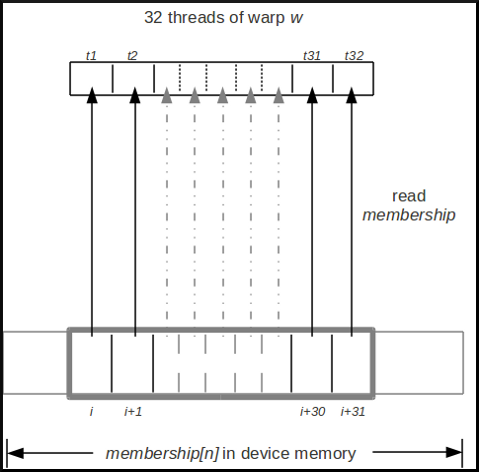
\includegraphics[width=0.45\textwidth]{./Data/intra_block_reduction/loadMembership}  	\label{fig:redcn_load} }
   \subfloat[Store $isMember$]{	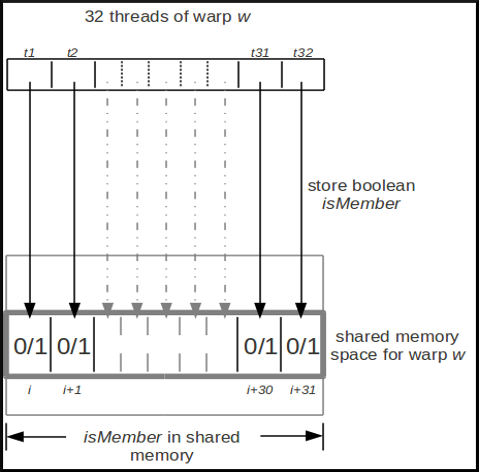
\includegraphics[width=0.45\textwidth]{./Data/intra_block_reduction/storeIsMember}  	\label{fig:redcn_store} }
   }

	\centerline{
   \subfloat[Find member]{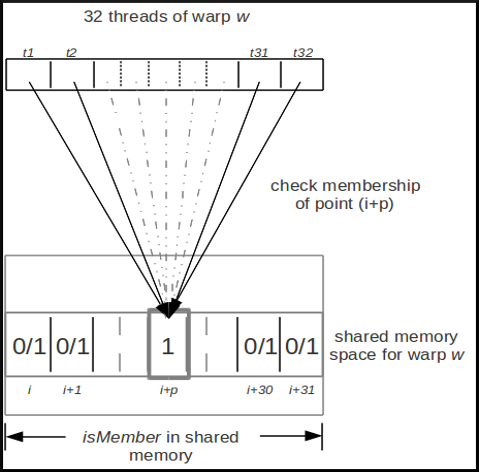
\includegraphics[width=0.45\textwidth]{./Data/intra_block_reduction/checkIsMember}  	\label{fig:redcn_check} }
   \subfloat[Add co-ordinates]{	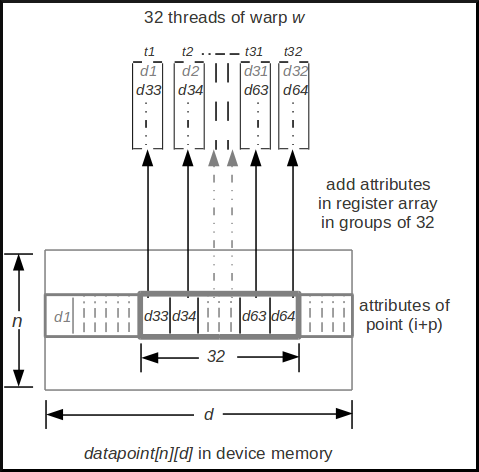
\includegraphics[width=0.45\textwidth]{./Data/intra_block_reduction/addDimensions}  	\label{fig:redcn_add} }
	}
	\caption{Illustration of intra-block reduction performed by a warp $w$ on data points $i$ to $i+31$. (a) Threads $t1$ to $t32$ load the $membership$ values for points $i$ to $i+31$. (b) Each thread stores boolean $isMember$ for corresponding data point into shared memory. (c) All 32 threads check value of $isMember$ for each point till they find point $i+p$ with value 1. (d) Successive co-ordinates of point $i+p$ are added by successive threads into their private arrays.}
\label{fig:redcn}
\end{figure}

\subsection{Reduce member co-ordinates}
This is the most crucial step as it involves maximum device memory reads. To ensure that co-ordinates of every member data point are read from device memory in a coalesced manner, separate reduction is performed by each warp inside the block. 

Data points to be processed by each block are partitioned equally among all the warps. Each warp processes its assigned data points without any dependence on threads from other warps as shown in Figure \ref{fig:redcn}. When all the points have been processed by every warp, they synchronize and the first warp reduces the $sum$ and $count$ values of all the warps.

Successive threads in a warp store successive dimensions of the reduced $sum$. Since the number of dimensions $d$ can be greater than 32, each thread has a register array of length $d/32$ to store reduced $sum$, where value at $i^{th}$ index, denotes the value of ($32*i+threadIdx.x$) dimension of the reduced $sum$; see Figure \ref{fig:redcn_add}. 

For every member data point, successive threads read and add the point's respective dimensions inside their private arrays.
This requires every thread in the warp to know which of the $32$ $membership$ indices were equal to $k$. Each thread stores value 0 or 1 inside a private register, $isMember$, to denote whether the the data point it checked is a member or not.
 
On C1060, value of $isMember$ is stored inside shared memory to communicate it with all the threads in the parent warp; see Figures \ref{fig:redcn_store} and \ref{fig:redcn_check}.
 
On Fermi based C2070, we use $\_\_ballot$ function to communicate the membership of data points within a warp without going through shared memory. Each thread invokes $\_\_ballot$ with argument $isMember$.
\begin{lstlisting}[morekeywords={__ffs}]
uint members = __ballot(isMember);
\end{lstlisting}

$\_\_ballot$ evaluates $isMember$ for all threads of the warp and returns an integer $members$ whose $N^{th}$ bit is set if and only if $isMember$ evaluates to non-zero for the $N^{th}$ thread of the warp. We find the non-zero bits inside $members$ by using $\_\_ffs$ function. $\_\_ffs$ returns the position of the first (least significant) bit set to 1 in $members$, where the least significant bit position is 1. Since, $\_\_ballot$ is only supported by devices of compute capability 2.x we could not use it on C1060.
\begin{lstlisting}[morekeywords={__ffs}]
while(members!=0)  {
// Find the position of first (least significant) bit set to 1
 int i = __ffs(members)-1;
 addDimensions(datapoint[i],sum);
 count++;
 // Clear the bit
 members = ((members >> (i+1))<<(i+1));
}
\end{lstlisting}
    
As shown by Figure \ref{fig:redcn_add}, successive threads need to access successive dimensions of the same data point. So the data points should be stored as $[n][d]$ inside device memory. But while assigning the clusters in Section \ref{sec:dataStorage}, they were required to be stored as [d][n]. To have data reads coalesced for both the cases we keep two copies of data points, one as $[n][d]$ and one as $[d][n]$ inside device memory.

\subsection{Store reduced values}\label{sec:storeReduced}
The final reduced values of $sum$ and $count$ are stored inside device memory. Each block stores its $count$ in an array in device memory at index $blockIdx.x$. The values of the reduced $sum$ are stored as $[K][b]$, where $b$ denotes the memory required for storing the reduced values of $sum$ for all the blocks assigned to the same cluster.

For each assigned cluster, every block stores all the dimensions of its reduced $sum$ at continuous memory locations. This helps coalesce the memory writes by each block.

\section{Inter-block Reduction}
After the completion of intra-block reduction, a separate kernel is invoked to reduce the values of $sum$ and $count$ that were stored for each cluster in Section \ref{sec:storeReduced}. One kernel block is created for each cluster and so the total number of blocks is equal to the number of clusters. Each kernel block reduces the values stored by all the blocks in Section \ref{sec:storeReduced} for the cluster $k$ assigned to it.
After reducing the $sum$ and $count$ values for cluster $k$, it finds the mean for every dimension. These means are the final co-ordinates of the centroid. 

Finally, each block stores the obtained co-ordinates of its centroid $k$, inside device memory.
